\section{COMPASS Data Structures}
\label{section:data_structures}

To enable spatial search, \emph{COMPASS} abstracts the infinite spatial complexity of the world into one of two concise representations- a location-centric structure or a concept map.
A \textit{location-centric structure} is a simple dictionary-based representation that describes a location by the objects contained in each of its four cardinal quadrants (Northwest, Northeast, Southwest, Southeast).
A \textit{concept map} represents a set of objects arranged spatially without explicitly encoding how they relate spatially to a location~\cite{Xu2010}.
Entries in the matrix either contain a $0$, representing empty space, or an object name, representing the position of that object.
Critically, concept maps are generated such that the relative order of objects from north to south and west to east is preserved from the original Cartesian representation, making them a condensed representation that captures the relevant spatial information needed to perform pattern matching.
Location-centric structures and concept maps can be generated from a pictorial query or a set of objects associated with a location. 
We implement concept maps using $N \times N$ matrices (where $N$ is the number of objects).
Figures~\ref{figure:ConceptMap-LO} and \ref{figure:ConceptMap} show the abstraction process used to create and search over these two data structures.

\subsection{Object-Location Data Structure}
Object-location relations encode cardinal directionality between objects and locations (i.e., whether an object is North, South, East, or West of a location). 
This type of information enables simple queries, such as when a user knows that a location has a lake on its western side. 
Each object-location relationship is defined independently of other objects associated with that location, and multiple constraints can be combined to form a more specific query, such as a lake west of the location and a pond south of the location.
Figure \ref{figure:ConceptMap-LO} shows how we encode a location (\ref{fig:CM-LO-Example}) as a geospatial index based on relative position to the location coordinates (\ref{fig:CM-LO-Setup}), and then how queries are processed (\ref{fig:CM-LO-Query}).
The search function returns the candidate locations ranked by the number of query terms that match the appropriate quadrant with respect to the location. 

\subsection{Object-Object ConceptMap Data Structure}
The other type of spatial relationships we support searching are object-object relations, which are typically more complex than object-location relations.
Object-object relations refer to a configuration of objects that relate to one another spatially.
For example, a tree, a pond, and a sign might form a triangle, with each object having a directional constraint to every other object in the query (i.e., tree upper left of pond, pond lower right of sign, and sign lower left of tree).
As the number of objects in the object-object configuration increases, the number of pairwise directional constraints needed to specify the query snowballs. 
Figure \ref{figure:ConceptMap} shows how we encode a location (\ref{fig:CM-Example}) as a matrix of relative object positions (\ref{fig:CM-OO-Setup}) and then how queries are processed (\ref{fig:CM-OO-Query}).
The object-object approach to defining spatial configurations of objects is also more flexible than the object-location approach, which requires the user to know where each object lies relative to the location. 


\begin{figure*}[t]
    \centering
    \begin{subfigure}[t]{.25\textwidth}
        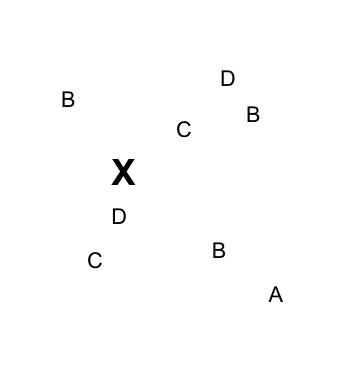
\includegraphics[width=\textwidth]{CM-ExampleLocation.png}
        \caption{\small A candidate location X has named objects A-D with the spatial layout depicted above.} 
        \label{fig:CM-LO-Example}
    \end{subfigure}
    \hfill
    \begin{subfigure}[t]{.25\textwidth}
        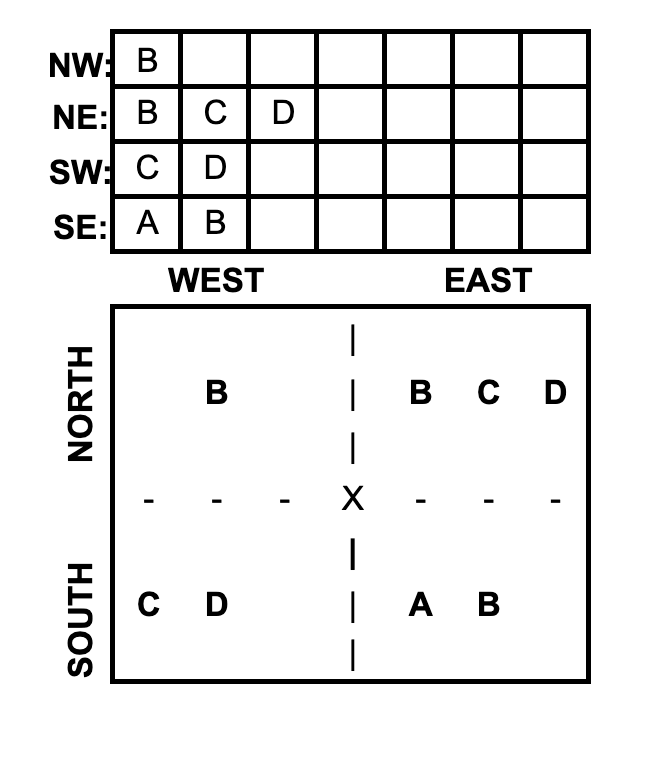
\includegraphics[width=\textwidth]{CM-LO-Setup.png}
        \caption{\small The objects are binned into spatial quadrants based on their relative position to the location coordinates, X.} 
        \label{fig:CM-LO-Setup}
    \end{subfigure}
    \hfill
        \begin{subfigure}[t]{.25\textwidth}
        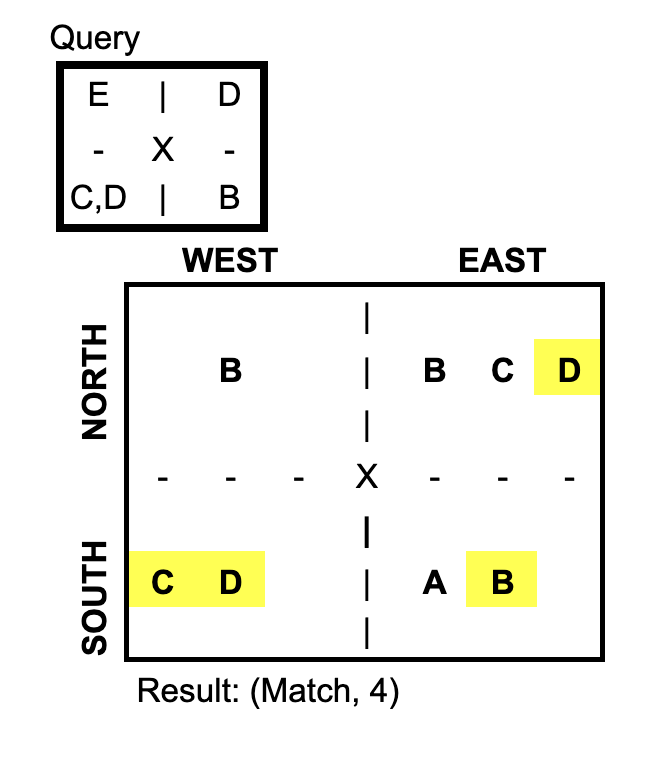
\includegraphics[width=\textwidth]{CM-LO-Query1.png}
        \caption{\small Rank the locations by the number of query terms that are found in the correct quadrant with respect to the location.}
        \label{fig:CM-LO-Query}
    \hfill
    \end{subfigure}
    \caption{\textbf{Object-Location Search Method. A Location-centric data structure (Figure \ref{fig:CM-LO-Setup}) is generated based on the cardinal relations between the objects and the location (Figure \ref{fig:CM-LO-Example}). Then a pictorial query is matched against the structure (Figure \ref{fig:CM-LO-Query}).}}\label{figure:ConceptMap-LO} 
\end{figure*}





\begin{figure*}[h]
    \centering
    \begin{subfigure}[t]{.25\textwidth}
        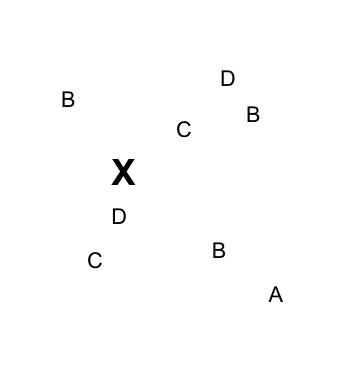
\includegraphics[width=\textwidth]{CM-ExampleLocation.png}
        \caption{\small A candidate location X has named objects A-D with the spatial layout depicted above.}
        \label{fig:CM-Example}
    \end{subfigure}
    \hfill
    \begin{subfigure}[t]{.25\textwidth}
        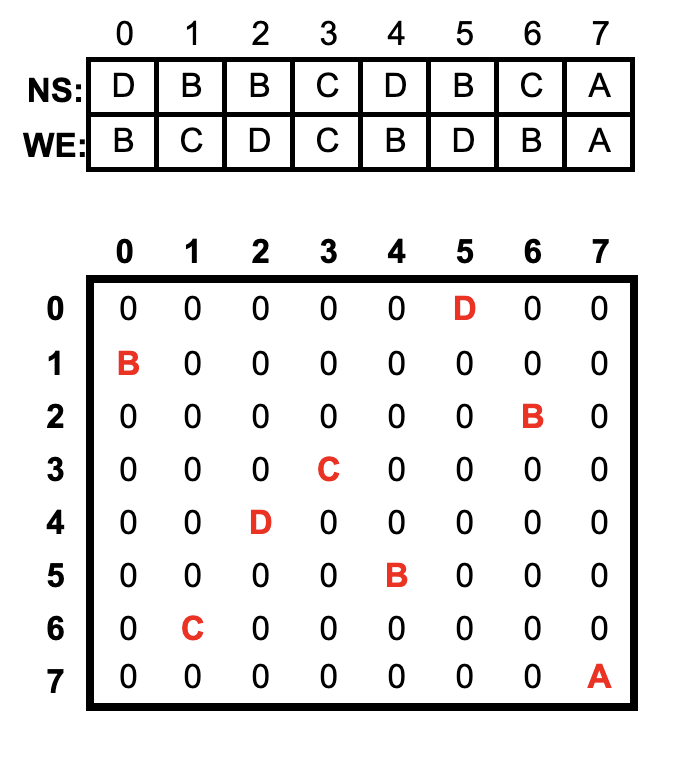
\includegraphics[width=\textwidth]{CM-OO-Setup.png}
        \caption{\small Objects associated with location X are ordered from North to South (NS) and West to East (WE) and mapped into a matrix with corresponding indices.}
        \label{fig:CM-OO-Setup}
    \end{subfigure}
    \hfill
        \begin{subfigure}[t]{.25\textwidth}
        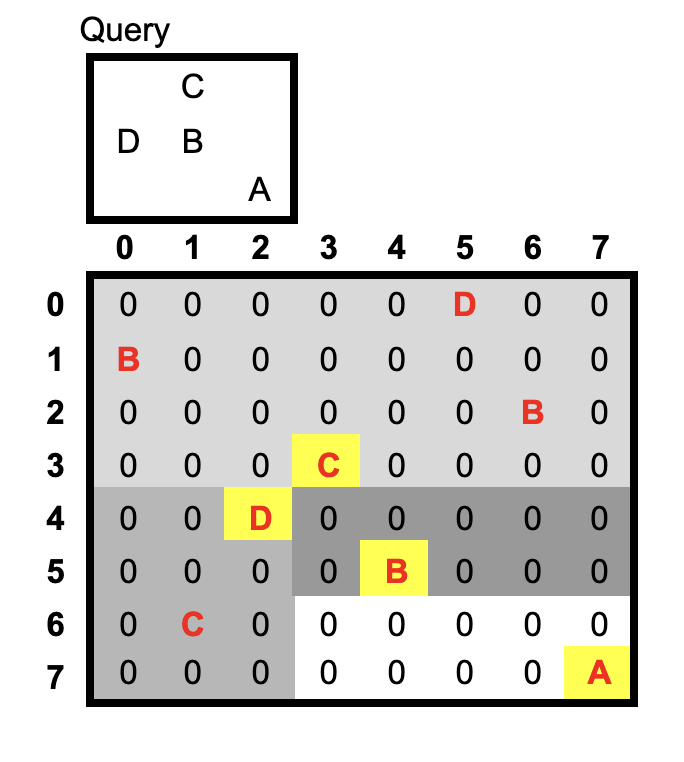
\includegraphics[width=\textwidth]{CM-OO-Query1.png}
        \caption{\small Recursive search. Each recursion is a darker shade, with an unpruned area in white. Objects highlighted in yellow are found to match the query configuration; candidate location X is a match for the query.}
        \label{fig:CM-OO-Query}
    \hfill
    \end{subfigure}
    \caption{\textbf{Object-Object Search Method. A Concept Map data structure (Figure \ref{fig:CM-OO-Setup}) is generated by ordering the objects associated with a candidate location (Figure \ref{fig:CM-Example}) from North to South and West to East. The search step (Figure \ref{fig:CM-OO-Query}) then recursively prunes the concept map until ANY matching configuration of objects is identified or the query constraints are not satisfied.
    }}\label{figure:ConceptMap} 
\end{figure*}